\newpage
\chapter{Обзор на игрите}
\label{chapter01}

“Stratego” представлява логическа игра характеризираща се с абстракцията, която от своя страна поражда аналитичното мислене в играчите. Логическите игри добиват наименование си поради структурата си, която се гради на точно определени правила създаващи интересни сценарий за играчите. Под формата на въпроси, екстремни тестове, задачи и други способи, като сравняваща оценка между участниците и това как реагират и действат в динамична ситуация. Текущите логически игри са разнообразни. По принцип всяка логична задача може да бъде "gamified" (да прилагат типични елементи на игра (например точкуване, съревнование с противника, правила на игра) към (дейност), обикновено като онлайн маркетингова техника за насърчаване на ангажираността с продукт или услуга), чието динамично взаимодействие тества основната идеята. 

\section{История на логическите игри}

\begin{lstlisting}
https://en.wikipedia.org/wiki/Logic_games
\end{lstlisting}

Логическите игри се разделят на няколко типа, които обстойно изучават семантиката и конструкцията и. Основният е линейният, тъй като съдържа два асортимента от променливи. Те наслояват променливите като ги съпоставят една с друга съгласно инструкциите на дадената игра. Следващият тип - разширено линеен е сходен на предходния, но броят на променливи се увеличава започвайки от три или повече променливи. При груповият вид концепцията се отклонява от стандартната,променливите са присвоени на групи като не се спазва определена последователност. Последният вид е съчетание между груповите и променливите.

Логическите игри биват характеризирани като специфични, тъй като следят разсъжденията и поведението на играчите в напрегната и несигурна ситуация, което прави играта по реалистична като изживяване, а на теория обогатява знанията и разширява гледната точка на участниците.

\subsection{Игри с открити условя}

\begin{lstlisting}
https://en.wikipedia.org/wiki/Perfect_information
https://en.wikipedia.org/wiki/Complete_information
\end{lstlisting}

\subsection{Игри с открити условя}

\subsection{Игри с неизвестност}

\section{Сложност на логическите игри}

\begin{lstlisting}
https://en.wikipedia.org/wiki/Game_complexity
\end{lstlisting}

\section{Играта Stratego}

Staratego” е бордова игра сходна на шаха, но с по-голяма сложност, която се изразява в обхвата на всички достижими конфигурации на всяка съществуваща бордова игра. Нивото на сложност е трудно за определяне, но теоретичното изчисление преброява всички позволени и не позволени позиции. Сложността се основава и на разликата понятията на незаконна конфигурация и недостижимата позиция. Незаконна конфигурация в „Stratego“ е в случаи при липса на двата флага върху дъска или когато двата флага са поставени един до друг. Позволената, но недостъпна позиция е бордова конфигурация върху дъската, където всички клетки са блокирани от бомби, но пионката е преминала през тях. В резултат на променливи празни клетки и отстранени пионки, може да се приложи доста по-сложна формула за изчисляване на сложността на пространството състоянието събирайки 12-те сини и 12-те червени пионки. Трябва да се взема предвид, че бомбите могат да бъдат поставени само в клетките на всеки играч, който по правилата на играта разполага с индивидуално поле при стартиране 4 × 10 и двамата играчи трябва да имат индивидуално знаме, което им позволява да бъдат на игралната дъска. Изчислението е осъществено с помощта на хеширани стойности за да намалят самото на времето за изчисление.

Когато се правят твърде сложни изчисления, чрез незаконни позиции или недостъпни  позиции. Като допълнение на сложността е включено и дървовидното разклоняване, което изчислява средният брой ходове на всеки играч. След 700 хода факторът на разклонението се увеличава и отново преминава към линейната сложност. Ако играта приключи преди разиграването на 700-те хода , действието на разклоняващият фактор намалява. Статистически погледнато средният фактор на разклоняване е приблизително 21.739, а играта има средно 30.363 случайни възли, където всеки случаен възел има среден разклонителен фактор от 6.823. С други думи, сложността на дървовидното разклонение е независима от стартиращата позиция.

\subsection{Правила на играта}

Основната цел на играта е един от играчите да завладее флага на противника по зададените правила за разиграване.

Началото на „Stratego“ се играе като предварително се определят териториите на участниците. Те разполагат с поле от 10x10 клетки между противниците са разположени две езера с размер 2x2 в средата на дъската. Играчите разпределят своите 40 пионки с гръб към противника на 4x10 области. Единият играч със сините пионки, а за другият остават червените, като пионките биват разпределени и поставяни по редици. Това става като се започне с поставянето на пионките с най-нисък приоритет до най-висок: шпионин, скаут, миньор, сержант, лейтенант, капитан, полковник, майор, генерал, маршал. Играчите разполагат и с два типа основно важни, неподвижни пионки: флаг и бомби.

След като двамата играчи разположат всичките си пионки, първи на ход е червеният играч, който може да избере дали да придвижи пионка или да атакува пионка на противника си.

Движения на пионките спрямо правилата: \\
-Алтернативни движения на пионките на синия и червеният играч; \\
-Пионките се преместват с един квадрат по ортогонално съседни свободни квадрати (скаутът е изключение от това правило); \\
-Забранени са движенията върху клетките на езерата, следователно мога да бъдат заобиколени със съседните им клетки; \\
-Само една пионка може да заема клетка; \\
-На всеки играч се полага по един ход на движение; \\
-Скаутите могат да бъдат местени на произволен брой свободни квадрати и да се движат както напред, назад или настрани (ляво/дясно).

Атакуване на противника:

\begin{lstlisting}
https://en.wikipedia.org/wiki/Stratego
\end{lstlisting}

\subsection{Оптимално първоначално подреждане}

\begin{figure}[h!]
 \centering
 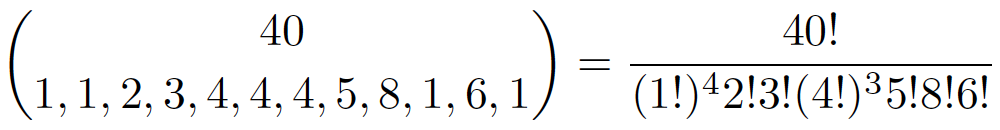
\includegraphics[width=1.0\linewidth]{fig01}
 \caption{Брой комбинации за първоначално подреждане на пионките \cite{arts01}}
\label{figure01}
\end{figure}
\FloatBarrier

\begin{lstlisting}
http://www.ultrastratego.com/setups.php
\end{lstlisting}

\subsection{Оптимално разиграване}

\begin{figure}[h!]
 \centering
 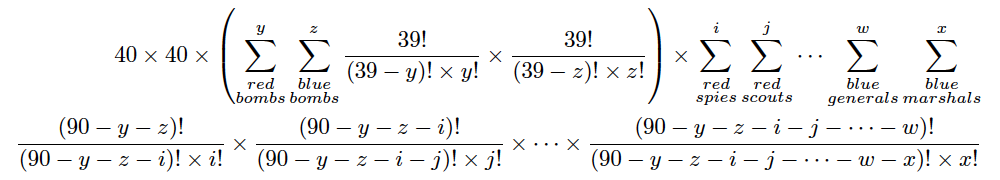
\includegraphics[width=1.0\linewidth]{fig02}
 \caption{Формула за възможните разигравания \cite{arts01}}
\label{figure02}
\end{figure}
\FloatBarrier

\begin{lstlisting}
http://www.ultrastratego.com/tactics.php
\end{lstlisting}

\section{Проблем, цели и задачи}

Логическите игри през вековете са имали за основна цел да развиват тактическите и стратегическите умения на различни хора в обществото (предимно военачалници). В наши дни логическите игри спомагат за развитие на умения при инвестиране или планиране. Също така логическите игри намират широко приложение като развлечение. С развитието на компютрите и мобилните устройства все повече класически игри (на дъска и не само) се реализират под формата на електронни игри и служат за уплътняване на свободното време. 

Настоящата дипломна работа адресира проблема свързан с развитието на логическото мислене при хората, на първо място и възможността за развлечения в моментите на скука, на второ място. 

Постигането на следните цели, поставени в дипломната работа водят до решаването на поставения проблем: \\
G.1 Разработка на електронна игра „Stratego“; \\
G.2 Разработка на възможности за реализация на изкуствен интелект в електронната игра; \\
G.3 Изследване на възможностите за различни стратегии;

Постигането на набелязаните в дипломната работа цели се осъществява, чрез изпълнението на следните задачи: \\
T.1.1 Изработване на графичен интерфейс за мобилно приложение на играта; \\
T.1.2 Изработване на обектно-ориентиран модел на електронната игра; \\
T.1.3 Изработване на релационен модел за съхраняване на информацията в играта; \\
Т.1.4 Изработване на програмен код за мобилна комуникация, така че играчите да имат възможност за игра в мрежа; \\
T.2.1 Съставяне на подходящи програмни модули за компютърен опонент; \\
T.2.2 Реализация на компютърен опонент по принципа „случайно търсене“ (Rrandom Search); \\
T.3.1 Реализация на изследване за оптимално първоначално подреждане на игралното табло с Монте Карло дървовидно търсене (Monte Carlo Tree Search); \\

